\documentclass[runningheads,a4paper]{llncs}

\usepackage[utf8]{inputenc}
\usepackage{graphicx}
\usepackage{listings, color}
\usepackage[bookmarks,bookmarksopen,bookmarksdepth=2]{hyperref}

\graphicspath{ {./img/} }



\begin{document}

\title{Traceability \& Mega-modeling}
\subtitle{An introduction for undergraduates}
\author{Maximilian Meffert}
\institute{University of Koblenz-Landau}
\maketitle
\begin{abstract}

Traceability and mega-modeling deliver a strong foundation to comprehend and work with big systems but neither of those concepts is part of an undergraduate curriculum in computer science. However graduation qualifies to work with even large systems. 
This paper introduces both ideas on an undergraduate level and exemplifies their beneficial combination by comparing three approaches alongside their targeted development phases.


\keywords{
traceability,
mega-modeling,
requirement engineering,
model driven engineering,
architecture frameworks,
runtime models
}


\end{abstract}


\section{Introduction}\label{sec:Introduction}
Software and computer systems tend to become bigger and more complex to meet higher expectations.
At the same time the complexity of engineering processes creating and maintaining such systems increases proportionally.
One way of taming this rising complexity is the concept of \textit{traceability} which is commonly interpreted as the system ability \textit{''... to describe and follow the life of software artifacts ...''} \cite{ScopedTraceability}, but it is not yet part of an undergraduate curriculum in computer science. 
Neither is \textit{mega-modeling} due to its high level of abstraction, as it deals with models using other models as their elements. 
We argue that it is reasonable for undergraduates to get familiar with both concepts regarding the fact that an achieved degree qualifies to work with even large systems.

In this paper we will outline the basics of traceability and mega-modeling on an undergraduate level, and show how the combination of both can be beneficial to engineers in terms of \textit{system understanding} and \textit{process management automation} so mega-modeling allows one to use model driven engineering (MDE) techniques and technologies.

\subsection{Contributions of this paper}
\subsubsection{Contributions}
\subsubsection{Non-Contributions}

\subsection{Road-map}\label{subsec:Introduction.Road-map}
§\ref{sec:BasicsOfTraceability}
introduces the concept in terms of terminology and motivation of traceability.
§\ref{sec:BasicsOfMegamodeling}
introduces the concept of mega-models.
§\ref{sec:TraceabilityObjectivesRevisited}
revisits traceability objectives and introduces a higher categorization.
§\ref{sec:TraceabilityMegamodels}
summarizes three approaches on traceability, mega-models and traceability mega-models.
§\ref{sec:Conclusion}
concludes the paper.



\section{Basics of traceability}\label{sec:BasicsOfTraceability}
Historically the research on traceability in software engineering originates from requirement engineering (RE). 
The question is: given a discrete set of requirements, how can one validate or even prove that all requirements are met? 
And more importantly on what information can one base such validation? 

The idea to solve this problem came through observation on typical product development processes where a raw vision is transformed to concrete requirements, requirements are transformed to architecture and architecture is transformed to a final implementation. 
Due to the incremental and iterative nature of such processes it is reasonable to assume that engineering activities might leave \textit{traces} which reflect the performed activity and the past state of the modified artifact.

Later traceability became of more interest to the MDE community. 
The purpose of traceability here did not much differ from its purpose in requirement or software engineering. 
We just change our perspective on how we see and describe engineering processes. 
Usually we try to regard artifacts as models of some kind at best specified by meta-models, and activities are seen as also well defined model-transformations. 
On top of that MDE is strongly interested in the automation of engineering processes.

Winkler and von Pilgrim compiled a complete survey on traceability where origins and differences in both fields can be explored in more detail \cite{TraceabilitySurvey}. 
This section is strongly based on their work.


\subsection{Traceability definitions}
Traceability is subject of various research fields, hence there is no standard definition on what traceability actually is. 
The introductory citation is from Lago et al. \cite{ScopedTraceability} and states the following: 
\textit{''Traceability is the ability to describe and follow the life of a software artifact and a means for modeling the relations between software artifacts in an explicit way''}. 
This definition is a good starting point if one wants to grasp what traceability is about because it is based on the life-cycle of artifacts and their relationships which has a nice intuitive notion. 
However, there is a weakness, it is not clear whose ability it should be. Other more technical definitions of traceability are given by the IEEE \cite{IEEEGlossary}:
\begin{enumerate}

\item 
\label{item:IEEEDef1}
\textit{The degree to which a relationship can be established between two or more products of the development process, especially products having a predecessor-successor or master-subordinate relationship to one another.}

\item 
\label{item:IEEEDef2}
\textit{The degree to which each element in a software development products establishes its reason for existing.}

\end{enumerate}
Here, traceability is not seen as an ambiguous ability, on the contrary it is stated as a hopefully measurable degree of relationships. 
Moreover in definition \ref{item:IEEEDef2} product elements are made accountable for their own traceability.


\subsubsection{traces}
Vital to traceability is the idea that engineering activities leave traces. 
Such traces may appear in form of meta-information describing hard facts like \textit{what} happened, \textit{who} did something or \textit{when} something happened. 
Opposing that traces also may appear as \textit{''... (non-) material indication or evidence ...''} \cite{OED} on \textit{why} or \textit{how} something happened. 

For example version control systems automatically record the user, modification date and the modification itself committed for a given artifact.
Additionally a commit-message is passed alongside which hopefully gives some insights on the stored changes.
These messages could refer to a customer interview, a discussion under colleagues or technical research to establish some reason on the modification. 
Such conversations are usually not transcribed, hence they are considered soft traceability information.
Note: the modification itself is also considered to reflect such non-material traceability information, although this data is hard to obtain unless there is explicit documentation like sufficient doc-comments or commit-messages.

Following this separation in hard and soft fact traces Pinheiro \cite{Pinheiro} defines a classification which somewhat resembles the separation commonly used on requirements:
\begin{itemize}

\item
\textbf{Functional traces:}
Traces existing due to well defined transformations. Such transformations produce traces as by-products like revision numbers in version control systems. Or traces that may be obtained by analyzing the transformation input, output and rules. In short, these traces have to obey some sort of formalism.

\item
\textbf{Non-Functional traces:}
Traces which cover \textit{''reason, context, decision, and technical''} aspects. I.e. explaining the informal interpretation of MUST and SHOULD in requirements.

\end{itemize}

\subsubsection{traceability links}
The IEEE \cite{IEEEGlossary} defines a trace as a record \textit{''To establish a relationship between two or more products of the development process; for example, to establish the relationship between a given requirement and the design element that implements that requirement.''}. 
The frequent notion of relationships describing or supporting traceability leads to the concept of \textit{traceability links}.
These links can be seen as a more technical description of traces as they are stated to be instances of  n-ary, multi-directional relations, although they are not named by the IEEE Glossary like traces and are often used as synonyms for one another \cite{TraceabilitySurvey}.
This can be misleading in environments which are not not strongly modeled where traceability links seem to not cover simple meta-data.

\begin{figure}
\centering
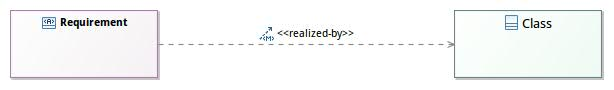
\includegraphics[width=\textwidth]{SimpleRealizationTraceabilityLink.jpg}
\caption{Requirement realization link}
\label{fig:RequirementRealizationLink}
\end{figure}

A simple example for traceability links is shown in Figure \ref{fig:RequirementRealizationLink} where the realization of a requirement by a class is denoted. 
However, this is a minimal example, in real-life the relation might need a higher arity to add constrains and test cases in order to confirm realization.

There are also categorizations on traceability links mostly considering the phase or abstraction nature.
For requirements engineering Gotel and Finkelstein use a big phase classification differentiating between \textit{pre- and post- requirement specification traceability} \cite{GotelFinkelstein}.
On the other hand Ramesh and Edwards distinct between \textit{horizontal and vertical traceability} \cite{RameshEdwards}.
Figure \ref{fig:RequirementRealizationLink} exemplifies vertical traceability as realization is a relation between abstraction layers.

Similar to these classifications there is \textit{pre-, intra- and post model traceability} by Paige et al. for MDD considering traceability between the first non-model artifacts and the first model, traceability during model-refinement and traceability between the final model and generated artifacts \cite{TraceabilitySurvey}.

Till now we introduced the mere concept of traceability which is far from applicable.
To make actually use of traces and traceability links we need do define schemes in RE or meta-models in MDD which also may vary with their targeted domain.
Traceability meta-models will be covered in a later section.


\subsection{Traceability objectives}
Another thing we like to point out besides the introduction to the rather theoretical concept of traceability is the motivation behind all this. 
Winkler and von Pilgrim \cite{TraceabilitySurvey} identified several objectives where traceability might be of great help. 
Figure \ref{fig:TraceabilityObjectives} depicts traceability objectives sorted by the research field they originated from. 
However most objectives found in requirements engineering can also be considered important to the MDD community. 
Additionally some objectives already correspond directly, i.e. \textit{Estimating change impact} and \textit{Change impact analysis} do not differ at all regarding their purpose. 
Given sufficient traceability information in form of traces and traceability links one can simulate changes top-down to the final model and estimate their impact on metrics like quality, performance, cost, etc. 
The only difference between RE and MDE here lies in the propagation of changes. 
Where in RE changes are considered to be propagated manually, MDE uses automation. 
Although nowadays RE also relies on tool support.

\begin{figure}
\centering
%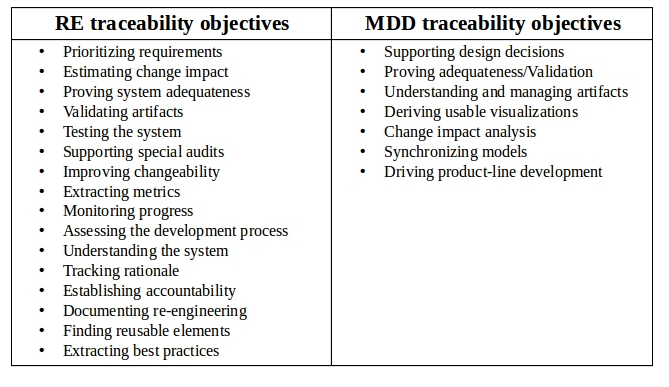
\includegraphics[width=\textwidth]{TraceabilityObjectives.jpg}
\begin{tabular}{|c|c|}
\hline
\begin{minipage}[t][][c]{0.5\textwidth}
\centering
\textbf{RE Traceability Objectives}
\end{minipage}

&

\begin{minipage}[t][][c]{0.5\textwidth}
\centering
\textbf{MDE Traceability Objectives}
\end{minipage}

\\\hline

\begin{minipage}[t][][c]{0.5\textwidth}
\vspace{0.1cm}
\begin{itemize}
\renewcommand{\labelitemi}{$\bullet$}

\item Prioritizing requirements 
\item Estimating change impact 
\item Proving system adequateness 
\item Validating artifacts 
\item Testing the system 
\item Supporting special audits 
\item Improving changeability 
\item Extracting metrics 
\item Monitoring progress 
\item Assessing the development process
\item Understanding the system 
\item Tracking rationale 
\item Establishing accountability 
\item Documenting re-engineering 
\item Finding reusable elements 
\item Extracting best practices 

\end{itemize}
\vspace{0.1cm}
\end{minipage}

&

\begin{minipage}[t][][c]{0.5\textwidth}
\vspace{0.1cm}
\begin{itemize}
\renewcommand{\labelitemi}{$\bullet$}

\item Supporting design decisions
\item Proving adequateness/Validation
\item Understanding and managing artifacts
\item Deriving usable visualizations
\item Change impact analysis
\item Synchronizing models
\item Driving product-line development

\end{itemize}
\vspace{0.1cm}
\end{minipage}

\\\hline

\end{tabular}
\caption{Traceability Objectives identified by Winkler and von Pilgrim \cite{TraceabilitySurvey}}
\label{fig:TraceabilityObjectives}
\end{figure}

Other corresponding objectives are \textit{Proving system adequateness}/\textit{Validating artifacts} and \textit{Proving adequateness/Validation}. 
If end-to-end traceability from early artifacts to the final implementation is achieved, one cannot only use traces to identify incompleteness (again top-down), it is also possible to check for requirement coverage (bottom-up).
This is especially beneficial for the use case to attest customers that the system specification is met and not exceeded.

Besides these product centric objectives which mainly address maintainability and soundness concerns of a completed project, there are also objectives to support the development process itself.
Such are \textit{Monitoring progress} and \textit{Establishing accountability} where project management can leverage end-to-end traceability to determine if a milestone is reached or who to blame if not. 

Eventually we can learn from collected traceability data during a project revision while \textit{Extract Best Practices} to support future design decisions. 




\section{Basics of mega-modeling}\label{sec:BasicsOfMegamodeling}
The second topic of current research on which we need basic knowledge to understand the coming sections is mega-modeling. The term mega-model is somewhat ambiguous as it commonly refers to models using other models as their elements. But the term model is not used in a restrictive manner \cite{MEGAL2}, it may be interpreted as intuitive models, elements of such models, meta-models describing such models and moreover the term may be used for mega-models itself as depicted in Figure \ref{fig:BoradSenseMegaModel}, so mega-models could actually describe mega-mega-models or even mega*-models. And to make things a little bit more confusing mega-models may also be defined by meta-models.

\begin{figure}
\centering
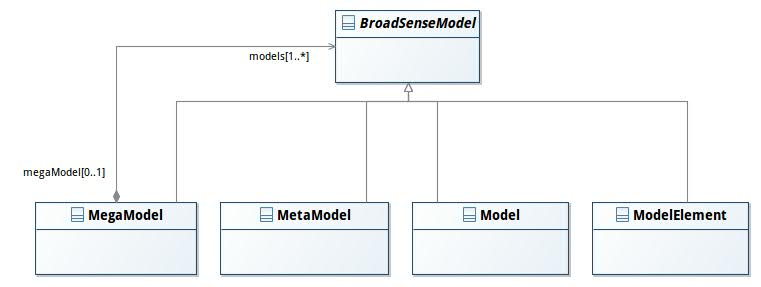
\includegraphics[width=\textwidth]{BroadSenseMegaModel.jpg}
\caption{Mega-models in a broad sense}
\label{fig:BoradSenseMegaModel}
\end{figure}

\subsection{Mega-model usage}\label{subsec:MegaModelUsage}
Unsurprisingly mega-models are meant to be used for large-scale modeling, i.e. models of big enterprise systems \cite{TowardsAMegamodel}. Such systems are ecosystem-like environments consisting of various different technologies interacting with each other. Especially regarding this aspect of systems one can make use of mega-models to investigate the dependencies of involved \textit{technological spaces} \cite{MEGAL1}\cite{MEGAL2}\cite{TowardsAMegamodel}. However the use of mega-models may not only be indicated by system size. Even minimal static \footnote{static in a sense that content data is not provided dynamically, i.e. form of databases} web-pages can use a multitude of technologies in form of
\begin{itemize}
\item software languages like HTML, CSS and JavaScript (nowadays CSS also may conform to corresponding LESS or SASS code),
\item software APIs likes JQuery, Angular.js, etc.,
\item infrastructure components like server and client/browser, 
\item and protocols like HTTP(S) or FTP.
\end{itemize}
Enhancing the web-page with server side logic might add the technological spaces of PHP-ware, Java-ware and/or SQL-ware.

Another use case or need for mega-models arises implicitly when one wants to build MDE supporting tools. MDE-tools provide functionalities to create and maintain digital representations of models, meta-models and model- transformations. To do so, such tools need to implement a meta-model capable of these three (ore more) aspects, whose object instances would in fact be some sort of mega-models. Seibel et al. \cite{DHMM} created a prototype which is able of managing traceability links between models and model-elements by utilizing a meta-mega-model.

\subsection{The MDE-Mega-Model}\label{subsec:TheMDEMegaModel}
One particular mega-model we want to point out is the MDE-Mega-Model (Figure \ref{fig:TheMDEMegaModel}) by Favre et al. \cite{TowardsAMegamodel}.This approach aims to model MDE evolution processes. Although it is not yet complete, it already proves to be a powerful help analyzing technological spaces. 

\begin{figure}
\centering
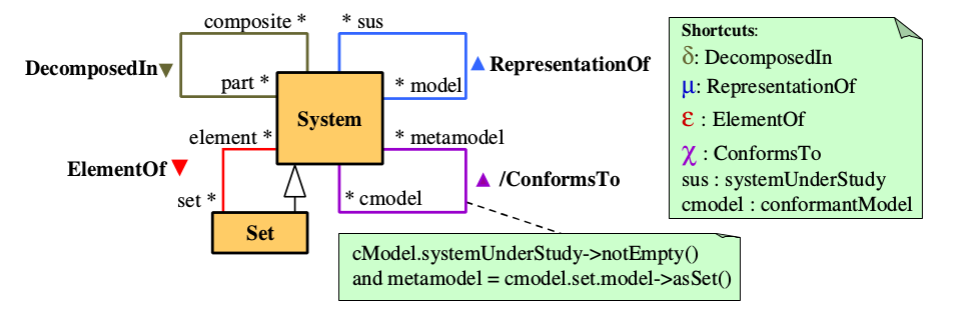
\includegraphics[width=\textwidth]{MDE-MegaModel.png}
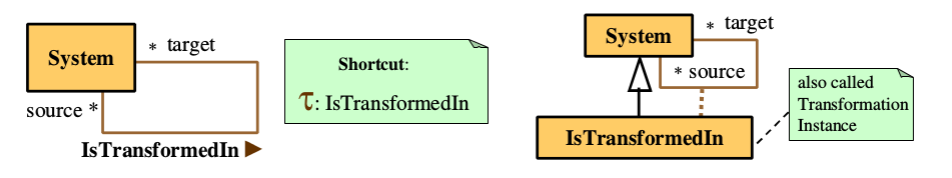
\includegraphics[width=\textwidth]{MDE-MegaModel-Transformations.png}
\caption{The MDE-Mega-Model by Favre et al. \cite{TowardsAMegamodel}}
\label{fig:TheMDEMegaModel}
\end{figure}

The other reason to introduce this mega-model here is due to its concise nature and high level of abstraction regarding MDE. This makes it an ideal framework for analyzing other concrete mega-models.

Favre et al. identify five relations concerning systems which we will now explain in short:

\subsubsection{systems} At first we need to clarify the term \textit{system}. Favre et al. state: \textit{''A system is the primary element of discourse when talking about MDE''}, although the terms usage may not be important as everything can be seen as some kind of system \cite{TowardsAMegamodel}. This is exemplified with the trigonometric system $\pi$ (meaning the real number). For the sake of simplicity and not repeating examples we may just think of a system as the \textit{thing of interest}.

\subsubsection{$\delta$ (\texttt{DecomposedIn})}
Decomposition is a structural relationship which denotes that a \textit{composite} can be \texttt{DecomposedIn} a \textit{part}, or in set-theoretic notation: 
\begin{center}
\textit{composite} $\delta$ \textit{part} or $(composite, part) \in \delta$
\end{center}
Example: A directory in a file system tree contains simple files and other directories, so its safe to say: \texttt{dir} $\delta$ \texttt{file} and \texttt{dir} $\delta$ \texttt{dir}. The latter also illustrates the recursive notion of this relation.

\subsubsection{$\mu$ (\texttt{RepresentationOf})}
Representation is a descriptive relationship denoting a \textit{model} as a \texttt{RepresentationOf} of a \textit{system under study}. We write:
\begin{center}
\textit{model} $\mu$ \textit{sus}
or 
(\textit{model},\textit{sus}) $\in\mu$
\end{center}
Again, we do not care that much about the term \textit{system}, for \textit{model} on the other hand we think of it as abstraction and/or simplification of such systems.
Example: As directories contain $n$ files, a list of files can be the representation of a directory: \texttt{[file0,file1,...]} $\mu$ \texttt{dir}.

\subsubsection{$\varepsilon$ (\texttt{ElementOf})}
This is simply the set-theoretic $\in$ relationship, so an \textit{element} is \texttt{ElementOf} a \textit{set}. In greek notation:
\begin{center}
\textit{element} $\varepsilon$ \textit{set}
or 
(\textit{element},\textit{set}) $\in\varepsilon$
\end{center}
Example: \texttt{FOO := (/foo)+}  may be the set of all Unix-files following the this pattern ( \texttt{FOO = \{ /foo, /foo/foo, /foo/foo/foo, ... \} } ), so \texttt{/foo} $\varepsilon$ \texttt{FOO}.

\subsubsection{$\chi$ (\texttt{ConformsTo})} Conformance adds the notion of meta-models, where a \textit{conformantModel} \texttt{ConformsTo} a \textit{metamodel}.
\begin{center}
\textit{cmodel} $\chi$ \textit{metamodel}
or 
(\textit{cmodel},\textit{metamodel}) $\in\chi$
\end{center}
Example: \texttt{(/foo)+} is a model for \texttt{FOO}, \texttt{/foo(/foo)*} is also one, so we have \texttt{(/foo)+} $\mu$ \texttt{FOO}. Both are regular expression describing the same set of strings and thus have to obey the syntax rules for regular expressions (\texttt{RegExp}), or in the notation of this mega-model: \texttt{(/foo)+} $\chi$ \texttt{RegExp}.

\subsubsection{$\tau$ (\texttt{IsTransformedIn})}
Transformations play a very important role in MDE because the benefit of just being able to statically describe systems is limited. Additionally we need the ability to model the progress of a development process. But this is relatively simple to achieve by applying the well known concept of functions to this mega-model. So we may say a \textit{source} \texttt{IsTransformedIn} a \textit{target}, we think \textit{source} $\mapsto$ \textit{target} and write:
\begin{center} 
\textit{source} $\tau$ \textit{target}
or 
(\textit{source},\textit{target}) $\in\tau$
\end{center}
Example: One transformation class of particular interest are model transformations. Given the established model \texttt{(/foo)+}, we might have it transformed to the model \texttt{(/bar)+}. This is denoted as  \texttt{(/foo)+} $\tau$ \texttt{(/bar)+} or (\texttt{(/foo)+}, \texttt{(/bar)+}). The latter is also called \textit{transformation instance/application}.
\newline

The MDE-Mega-Model and the important role of transformations and \textit{transformation systems} can be explored in more detail in the paper by Favre et al. \cite{TowardsAMegamodel}. It also offers some insights on the correlation of (formal) languages and models, which enables a higher point of view on software in general. However, for this paper and its discussion of traceability the short introduction above is sufficient.


\section{Traceability mega-models}\label{sec:TraceabilityMegamodels}
So far we discussed traceability and mega-modeling separate from one another in a rather abstract manner. From here upon out we will combine both by studying several real-life approaches. However, the set-theoretic notion of the MDE-Mega-Model in §\ref{subsec:TheMDEMegaModel} might have already revealed the connection between both topics. 

\subsection{MDE traceability}
MDE needs formalization in order to handle traceability properly. But the definition of traces alone does not work well with automation. Therefor the concept of \textit{traceability links} was introduced. Aizenbud-Reshef et al. define such links as \textit{''[...] any relationship that exists between artifacts involved in the software-engineering life cycle. [...]''} \cite{ModelTraceability}. Regarding models we have seen those relations in action:
\begin{center}
$a R b$
or
$(a,b) \in R$
\end{center}
This is the formalization utilized by the MDE-Mega-Model. We call the latter tuple representation a \textit{relation instance}. Such instances denote a mapping or \textit{link} between model-elements (modeled artifacts). So in fact the relations can be interpreted \textit{traceability link models} and the corresponding instances as actual \textit{traceability links}.

The MDE-Mega-Model defines only five relations, hence it is limited in inherent traceability. But this is sufficient due to its high level of abstraction and its objective to only model the fundamental relations to MDE. This set of relationships can easily be extended with additional traceability link models to achieve a higher degree of traceability. 

\subsection{MEGAF Architecture Frameworks}\label{subsec:ArchitectureFrameworkMegaModels}
MEGAF\footnote{\url{http://megaf.di.univaq.it}} is an approach on global model management by Hillard et al. \cite{MEGAF} utilizing mega-models to create reusable definitions of \textit{architecture frameworks}.

\begin{figure}
\centering
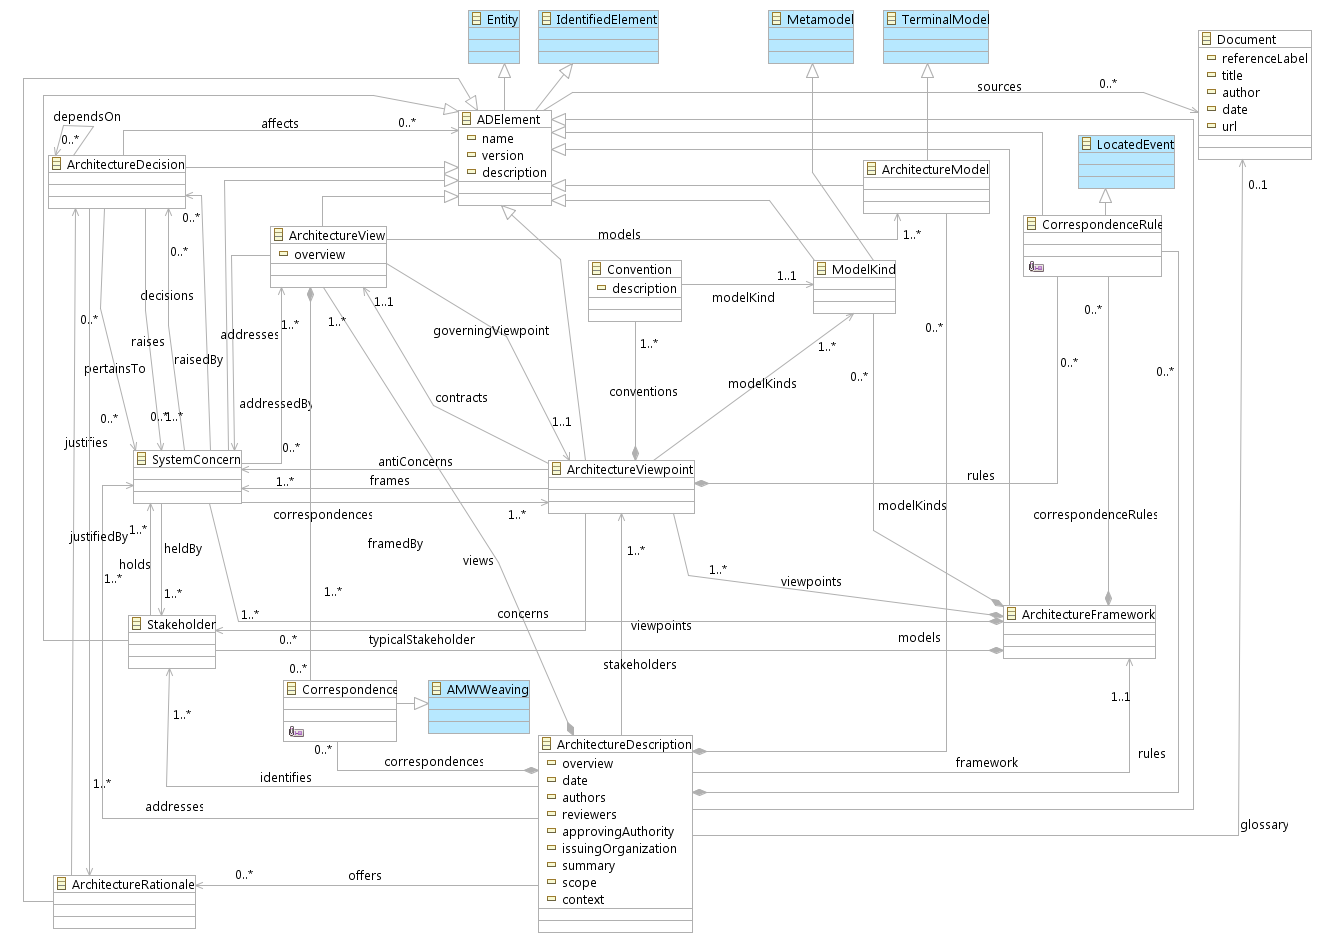
\includegraphics[width=\textwidth]{GMM4SA.png}
\caption{The GMM4SA meta-model}

\label{figure:GMM4SA}
\end{figure}

Architecture frameworks as defined by the \textit{ISO/IEC 42010 Software and System Engineering – Architecture Description} \cite{ISO/IEC42010} standard are collections of coordinated viewpoints, conventions, principles and practices to create architecture descriptions for specific stakeholders. Where \textit{architecture viewpoints} are collections of conventions, notations and modeling practices used to create concrete views which address domain specific system concerns for a distinct set of stakeholders. Their purpose is to capture and formalize a certain perspective.

According to the creators of MEGAF such architecture descriptions or frameworks alone have proven to be difficult to re-use and validate (consistency check). So in order to fix those issues, MEGAF shall provide features to: 
\begin{itemize}

\item 
\textit{store} architecture description elements (i.e. viewpoints, views, stakeholders, models, etc.), therefore making such elements reusable

\item
\textit{define correspondence relations and correspondence rules} between architecture description elements

\item
\textit{enable correctness and completeness checks} for architecture descriptions elements

\end{itemize}

To utilize mega-modeling techniques the assumption is made, that any architecture description element may conform to its meta-model. So a view may conform to a viewpoint, an architecture model may conform to a model kind, etc. This is straight forward and complies with the MDE world. The core of MEGAF is specified in \textit{Global Model Management for Software Architecture} (GMM4SA\footnote{\url{http://megaf.di.univaq.it/images/GMM4SA.png}}) meta-model shown in figure \ref{figure:GMM4SA} as UML class diagram. 

The diagram can be used to study the possible traceability of MEGAF. Because it is written in UML syntax, UML semantics apply and we already can identify several traceability links known from the MDE-Mega-Model. For example:
{\small \texttt{ArchitectureFramework} $\delta$ \texttt{ArchitectureViewpoint}} or {\small \texttt{ArchitectureViewpoint} $\varepsilon$ \texttt{ADElement}}.
These relations exist inherent in class diagrams as association/aggregation/composition ($\delta$) and generalization\footnote{UML generalization and realization do not map precisely to $\varepsilon$ and $\chi$ . The meaning may vary with the employed perspective. The set theoretic perspective ($\varepsilon$) might be used for data modeling. The model-meta-model perspective ($\chi$) might be used to describe inheritance or interface realization.} ($\varepsilon, \chi$). But this is trivial traceability information. The more beneficial traceability information here lies within the modeled context and intention. Because architecture description elements (children of \texttt{ADElement}) are formalizations of development process artifacts, all specified associations define a concrete traceability relation.

Lets consider the \texttt{ArchitectureViewpoint} class and its relations. In figure \ref{figure:GMM4SA} we see on the right hand side that \texttt{ArchitectureViewpoint} $\delta$ \texttt{Convention} and \texttt{ArchitectureViewpoint} $\delta$ \texttt{ModelKind}. Those are hard facts and can be interpreted as \textit{functional traces}. However on the left hand side wee see that an \texttt{ArchitectureViewpoint} \textit{frames} a \texttt{SystemConcern}. In the object oriented programming way of understanding such diagrams we would say \textit{frames} $\equiv \delta$. But if we also take the modeled context and intention of MEGAF into account, we discover how a \texttt{SystemConcern} traces to its holding \texttt{Stakeholder}, its pertaining \texttt{ArchitectureDecision} and the justifying \texttt{ArchitectureRationale}. Now we have information about \textit{reason, context and decision} and a successful formalization of \textit{non-functional traces}.

Wee see, the MEGAF meta-model supports traceability. Furthermore MEGAF and architecture frameworks in general target an very early phase of the development process. Using the higher order classification by Paige et. al \cite{}, MEGAF enables \textit{pre-model} traceability. However we need to note that pre-model traceability is concerned with non-model- to early-model-artifact traceability. On the other hand MEGAF seems to heavily discourage the use of non-model-artifacts at all. 


\subsection{Dynamic hierarchical mega-models \& Models at Runtime}
\subsection{Linguistic Architecture Analysis with MegaL}
MegaL\cite{MEGAL1}\cite{MEGAL2} is an approach on system understanding mainly concerned with the \textit{linguistic architecture} of the system under study. It intents to uncover the systems technological footprint by revealing the used technological spaces and their interrelations. This is called a \textit{linguistic} architecture because technological spaces of great interest are programming languages and their associated products.

In order to conduct a sufficient analysis MegaL needs to process the studied system against the 




%Favre et al. identify five key relations to MDE. According to the IEEE which regards traceability mainly established in form of relationships, all instances of such mega-model relations are hidden traceability links. Hence the identified mega-patterns by Favre et al. are all traceability patterns at a higher level.
%
%\section{Traceability objectives revisited}\label{sec:TraceabilityObjectivesRevisited}
%Although \textit{Understanding the system} is identified as a specific traceability objective, all objectives have dependent aspects from a MDD perspective. If we want efficient tool support regarding automation at first we need to have basic knowledge on how a system works, hence some high level objective can be considered \textit{System understanding}
%
%
%Recovered traceability links from MegaL \texttt{conformsTo} relations are transformation instances by Favre as a link $(artifact1,articaft2)$ means $artifact1~\tau~artifact2$ has been applied and therefor a transformation $\tau$ exists.




\section{Conclusion}\label{sec:Conclusion}

Conclusions are here.

\appendix
%\section{GMM4SA}

\begin{verbatim}
ADElement
ArichtectureDecision
ArchitectureDescription
ArchitectureFramework
ArchitectureModel
ArchitectureRelationale
ArchitectureView
ArchitectureViewpoint
Convention
Correspondence
CorrespondenceRule
Document
ModelKind
Stakeholder
SystemConcern

//===================================================

ArichtectureDecision dependsOn ArichtectureDecision
ArichtectureDecision justifiedBy ArchitectureRelationale
ArichtectureDecision pertainsTo SystemConcern
ArichtectureDecision raises SystemConcern
ArichtectureDecision affects ADElement

//===================================================

ArchitectureDescription identifies Stakeholder
ArchitectureDescription addresses SystemConcern
ArchitectureDescription offers ArchitectureRelationale

//===================================================

ArchitectureRelationale justifies ArichtectureDecision

//===================================================

ArchitectureView models ArchitectureModel

\end{verbatim}

\begin{thebibliography}{1}

\bibitem{DHMM}
A. Seibel, S. Neumann, and H. Giese. Dynamic hierarchical mega models: com- prehensive traceability and its efficient maintenance. Software \& Systems Mod- eling, 9(4):493–528, 2010.

\bibitem{IEEEGlossary}
IEEE: IEEE Standard Glossary of Software Engineering Terminology, IEEE Std 610.12-1990

\bibitem{MEGAL1}
Jean-Marie Favre, Ralf Lämmel, and Andrei Varanovich. Modeling the Linguistic Architecture of Software Products.

\bibitem{MEGAF}
R. Hilliard, I. Malavolta, H. Muccini, and P. Pelliccione. Realizing Architecture Frameworks Through Megamodelling Techniques. In Proc. of ASE’10, pages 305–308. ACM, 2010.

\bibitem{MEGAL2}
Ralf Lämmel and Andrei Varanovich. Interpretation of Linguistic Architectur. Unpublished, 2014

\bibitem{TraceabilitySurvey}
S. Winkler and J. von Pilgrim. A survey of traceability in requirements engineer- ing and model-driven development. Software and System Modeling, 9(4):529– 565, 2010. 

\bibitem{MegaRuntime}
Thomas Vogel, Andreas Seibel, and Holger Giese. The Role of Models and Megamodels at Runtime.

\bibitem{ScopedTraceability}
Lago, P., Muccini, H., van Vilet, H.: A scoped approacht to traceability management. J. Syst. Stoftw. 82(1), 168-182 (2009)

\bibitem{TowardsAMegamodel}
J.-M. Favre and T. NGuyen. Towards a Megamodel to Model Software Evolution through Transformations. ENTCS, 127(3), 2004. Proc. of the SETra Workshop.

\bibitem{Pinheiro}
Pinheiro, F.A.C.: Requirements traceability. In: Sampaio do Prado
Leite, J.C., Doorn, J.H. (eds.) Perspectives on Software Require-
ments, pp. 93–113. Springer, Berlin (2003)

\bibitem{GotelFinkelstein}
Gotel, O.C.Z., Finkelstein, A.C.W.: An analysis of the require-
ments traceability problem. In: 1st IEEE International Require-
ments Engineering Conference (RE’94) Proceedings, pp. 94–101.
IEEE Computer Society, New York (1994)

\bibitem{RameshEdwards}
Ramesh, B., Edwards, M.: Issues in the development of a require-
ments traceability model. In: Proceedings of the IEEE Interna-
tional Symposium on Requirements Engineering, pp. 256–259.
IEEE Computer Society, New York (1993)

\bibitem{OED}
Simpson, J., Weiner, E. (eds.): Oxford English Dictionary, vol. 18,
2nd edn. Clarendon Press, Oxford (1989). ISBN 978-0-198-
61186-8

\bibitem{ModelTraceability}
Aizenbud-Reshef, N., Nolan, B.T., Rubin, J., Shaham-Gafni, Y.:
Model traceability. IBM Syst. J. 45(3), 515–526 (2006)

\bibitem{ISO/IEC42010}
ISO. ISO/IEC CD1 42010, Systems and software engineering
— Architecture description (draft), January 2010.

\end{thebibliography}

\end{document}